% \section{Motivation}


\section{Related Work and Challenges}
\label{sec:related-work-challenges}

\ToStartMyDay{Start Writing \& Researching}

% Brief introduction to the section
This section provides an overview of the relevant work in the area of [briefly describe the broad area or field of study], with a particular emphasis on CIRCT (Circuit IR Compilers and Tools). We explore key features of CIRCT, the challenges they pose in the context of [your research area], and how our research addresses these challenges.

% Dedicated subsection for CIRCT and its features
\subsection{CIRCT: Circuit IR Compilers and Tools}

% \paragraph{Introduction to CIRCT}
CIRCT, or Circuit IR Compilers and Tools, represents [give a brief introduction of CIRCT]. It plays a crucial role in [explain its importance in your field or study].


% Thus, we can say that the hardware representations are not executable and need a simulator to stimulate them. This leads us to think about what the semantics of hardware representations look like. First of all, it should be executable and easy to use, like normal simulators, for validation. And it's vague, complicated and even impossible to construct circuit synthesizers for each dialect (using formal circuit representations to denote the semantics) since a single dialect even cannot construct a complete circuit. Thus, it sounds more reasonable to construct the semantics via capturing the behavior of the operations in the dialects. 

% 或许先讲目前的主要工作是怎样的，然后CIRCT project有什么全新的需求，这种challenge使得我们需要考虑一种novel的方式以应对这种问题。
% 有做的好的，有做的不好的。反正都写上去。有些好的，就可以在下面写solution的时候把insight放进去。
\begin{enumerate}
    \item \ToOpt{\textit{Intrinsic Extensibility} poses the first challenge in formalizing CIRCT. Rooted in the MLIR framework, CIRCT is capable of incorporating various intermediate representations through MLIR's extensible architecture, particularly through MLIR dialects. These dialects, revolving around a unifying ``operation'' concept, allow for a broad spectrum of semantics to be captured, diverging from the fixed constructs of traditional languages such as statements and instructions. This inherent flexibility, while a strength, also put forward more requirements for the formalization, including unified formalizations to one-to-one map to all the unified concepts in CIRCT, keeping each dialect formalization independently definable and exist, as well as their compatibility and composability with each other. Not only that, CIRCT, a framework for hardware, distinct itself from LLVM and MLIR's initial design objectives, further complicating the formalization.}
    
    \textit{Existing Efforts}. \ToPreWork{1. Research on semantics composability. 2. Summary them in Related Work.} \ToWrite{(1)before don't care, since no need. recent work on compatibility since llvm, mlir (2)composability: game semantics \& effect handler. more? (3) work on mlir/llvm. (4) what's the gap? theoretically? Technology? In terms of implementation?} \ToResearch{Game Semantics}. \ToResearch{Effect Handler} \ToCite{Reasoning about MLIR Semantics through Effects and Handlers} \ToRead{Modular, compositional, and executable formal semantics for LLVM IR} \ToRead{Interaction trees: representing recursive and impure programs in Coq} \ToWrite{Ours: 1. Extensibility. 2. Hardware.} % 由于PL的发展，近期对于可组合性的谈论不断增多。Existing work 可以不考虑组合性问题（虽然有工作做），因为他们需要描述的语言可能是成熟且确定的，并且仅仅是一个语言，不需要去考虑可组合性问题。然而。甚至目前的一点点在MLIR形式语义上的工作都没有考虑到可组合性的问题。或者说没有把可组合性当作一个专门需要讨论的问题。
    \item \DateMark{2024-01-08}{To Write the following} \textit{Accessible Executability.}  Different from representations for software which are initially designed for execution, the representations for hardware are designed for circuit synthesis and description. Even ISAs like x86 or ARM are also designed for execution since they are compiled from the software programs and just requirements for the hardware. Thus, the semantics of hardware representations can be a translation from HDLs to circuit descriptions, which makes it hard to validate the correctness of the semantics. 
    
    \textit{Existing Efforts}. \ToResearch{Like Yosys... Recent works notice the importance of hardware simulation, including ... Some ... Some ... However, existing works are not keen on the accessibility of the formal semantics, which adapts to hardware designers' knowledge domain and is crucial for the adoption of the formal semantics.}
    % The existing works on formalizing hardware representations also meet this challenge, and they ??? % 时序特征的处理 % 仿真/可执行方面的处理。（或许需要读一下verilog形式语义方面的工作，特别是essense of verilog） % 然而，他们。。。。 % 我们希望探索和已有simulator近似的接口，将形式语义和一般人/硬件开发人员熟悉的语言结合，使形式语义不仅仅可以作为一个规范，而十分容易获取。 % 此外，与他们的目标语言不同。CIRCT中每一个dialect无法单独构成硬件的描述，而是需要组合起来。每个硬件描述仅仅负责描述硬件的一个方面。 % 硬件语言特征和软件语言特征的区别。时序。同样用K描述他的语义的时候也是有区别的。最后做仿真的时候也是有区别的。 % 时序这一方面是不一样的，这些语义重点去写。 % 用K描述硬件的语义和软件的语义是有一些差别的。描述的是电路的结构，是不会执行的，需要一些激励才会执行。在做仿真的时候，怎么去做硬件的激励和仿真？需要一个很好的interface。
     % C的符号执行和gcc还是比较像的。硬件的符号执行可能会有一些其他的问题。写越底层的程序，性能是一个很大的问题。
     % It necessitates altering the Kore language, which can be challenging to understand and modify, to enable continuous stimulation. Furthermore, its output does not comprise VCD files.
    \item \textit{Early Stage.} CIRCT is a new project and is still in its infancy. Although it is already used by some novel languages and maintained by the LLVM community, the flaws in the documentation and the modification of the infrastructure are inevitable. \ToThink{This not only requires the extensibility but also requires an essence of CIRCT as a stable and reliable foundation.} 
    
    \textit{Existing Efforts}. \ToResearch{CIRCT does have a core dialect set inside of its documentation, while as a baby project even without a research paper, the described core dialect set is not the real essence of it. (1) Existing work on formal semantics is basically working on mature languages that are more mature in terms of documentation, communities, etc. (2) (this maybe set in insight) Recent works ($\lambda_x$) present xxx, which is a good start. However, it is not enough for CIRCT.}
    \item \textit{Ambiguous Documentation.} The flaws in the language reference are not the only problem. Although the CIRCT project continues the LLVM/MLIR project's emphasis on documentation and maintains the same documentation standards as MLIR. As a usability-first compiler project, they write documentation for the people who want to contribute to it, rather than who want to use the languages. So the CIRCT dialects explanation is ambiguous and not enough from the perspective of formalization. For example, the \textit{hw.module} operation even misses the syntax and semantics explanation. This requires the formal semantics to be able to fill the gaps in the documentation. % 如果仅仅是early stage似乎还没有那么难，但是充满不确定性的文档带来了更大的难度。即便MLIR已经定义的标准的文档格式，和ref生成手段，但是。。。
    
    \textit{Existing Efforts}. \ToResearch{Almost all the language formalization faces this challenging ambiguity. This became particularly prominent after LLVM designed IR (intermediate representations) for compilation purposes, leading to a kind of transparent language for normal programmers. This trend has continued to increase with the birth of languages such as Rust, and thus MLIR has emerged. This trend of separation is such that we currently don't even have a formal semantics that claims to formalize MLIR. only set of MLIR dialects or Theoretical Framework for MLIR. As a hardware compilation architecture, CIRCT further extends its complexity. This is due to the dual design goals of simulation/synthesis, which can be seen from the characteristics of HDLs such as Verilog.}
    \item \textit{Comprehensive Validation} is inseparable from a well-designed test set. The existing test in CIRCT is mainly focused on transformation and compilation, with few semantic targeted tests in the CIRCT test suite. \ToThink{Moreover, the existing tests from simulators or compilers for other languages like Verilog may not cover the features of CIRCT's essence, because of the language differences. Despite the correctness, it is also challenging to validate the completeness of the essence wether it is indeed sufficient to describe actual circuits.}
    
    
    \textit{Existing Efforts}. \ToResearch{Other formal semantics work. especially K.} % 目前大部分都是Verilog的测试用例， % 并不完全一样。
\end{enumerate}


% Discussing each feature, associated challenges, existing efforts and your solution
% - Introduction to the feature
% - Elaborating on its significance or applications
% - Transition to the challenge
% - Existing efforts and their limitations
% - Introduction to your solution
% - Detailing how your solution addresses the challenges
\subsubsection{Intrinsic Extensibility}
\ToWrite{Feature Overview}
Intrinsic extensibility in CIRCT is characterized by [describe the feature]. It is foundational for [explain its significance or applications].
\ToWrite{Challenge}
However, this feature introduces specific challenges, such as [list or describe the challenges]. These challenges primarily arise from [explain reasons behind these challenges].

\paragraph{Existing Efforts on Semantics Extensibility}
\ToWrite{Game Semantics... Effect Handler... Existing MLIR Semantics...}
Previous efforts in addressing intrinsic extensibility include [briefly describe existing efforts]. These approaches, while effective, have limitations like [mention limitations or gaps].

\paragraph{Existing Efforts on MLIR Semantics}

\ToCheck{This paragraph is copied from Related work} \textbf{Other Semantics of MLIR}. \citet{bangSMTBasedTranslationValidation2022} encodes memref dialect, linalg dialect, and dialects for tensors in SMT to deliver translation validation for machine learning compilers. Since they focus on a specific set of mature dialects, they do not provide modular and compositional semantics, as well as a unified approach to formalize dialects for extensibility. Furthermore, the semantics in SMT are not executable, which means that the semantics cannot be validated by co-simulation, leading to reduced confidence in the semantics. 
% 没有发论文的工作是不是就不用管了？mlir semantics

\ToCheck{This paragraph is copied from Related work} \textit{Comparison}. In contrast, for adapting to the ongoing hardware compiler infrastructure and facilitating future works on the MLIR formal semantics, Section~\ref{sec:semantics-formalization} presents a stratified semantics that is modular and compositional, as well as a unified approach in Section~\ref{sec:circt-static-semantics} to define the operation semantics which is the key to the dialect semantics. In addition, we propose a co-simulation framework to validate our executable semantics to build confidence in the correctness of the rules of the semantics and the completeness of the semantics to capture real-world hardware.

\paragraph{Our Solution}
\ToWrite{}
In contrast, our approach offers [describe your solution]. This method stands out due to [explain the uniqueness or effectiveness of your solution].


% Repeat the pattern for other features and challenges
\subsubsection{Accessible HDL Semantics}
\ToWrite{Feature Overview}
Intrinsic extensibility in CIRCT is characterized by [describe the feature]. It is foundational for [explain its significance or applications].
\ToWrite{Challenge}
However, this feature introduces specific challenges, such as [list or describe the challenges]. These challenges primarily arise from [explain reasons behind these challenges].

\paragraph{Existing Efforts on HDL Semantics Accessibility}

\paragraph{Existing Efforts on Semantics Accessibility}
\ToWrite{}
Previous efforts in addressing intrinsic extensibility include [briefly describe existing efforts]. These approaches, while effective, have limitations like [mention limitations or gaps]. \ToThink{A list is better?}


\paragraph{Existing Efforts on HDL Semantics}
\ToCheck{This paragraph is copied from Related work} \textbf{Other Semantics of Hardware Design Languages (HDL)}. Due to the growing diversity of hardware requirements, many hardware design languages, including Chisel\red{cite}, Bluespec\red{cite}, VHDL\red{cite}, and System Verilog\red{cite}, are proposed. Indeed, this diversity motivates the CIRCT project. Since formal verification requires formal semantics of HDL and plays a crucial role in ensuring the correctness of hardware, each HDL has at least one formal semantics. Thus, for clarity, the following merely discusses part works on the semantics of the most famous HDL --- Verilog\red{cite}.

\ToCheck{This paragraph is copied from Related work} Yosys~\cite{wolfYosysaFreeVerilog2013} is a open-source framework for RTL synthesis tools, which also support formal verification for extensive Verilog-2005. Therefore, it provides the semantics of Verilog by translating them into the logic network in AIGER or BLIF. After that, the hardware model checkers can verify formal properties on the given design. This a good way for formal verification, but the formal semantics are not executable which can be validated, too.  

\ToCheck{This paragraph is copied from Related work} \citet{meredithFormalExecutableSemantics2010}, in contrast, presents a formal executable semantics of Verilog in Maude. This semantics covers almost complete features of Verilog, but it fails to validate the correctness of the semantics. Furthermore, even though it builds upon the rewriting logic, which is a previous version of matching logic the logical foundation of the K framework, its implementation cannot be used in the modern K, leading to limited applications. \citet{khanVeriFormalExecutableFormal2017} introduce an executable formal model of Verilog in Isabelle/HOL, which also lacks a user-friendly interface and comprehensive co-simulation to validate the correctness of the formal semantics. 

\ToCheck{This paragraph is copied from Related work} \citet{chenEssenceVerilogTractable2023}, as the most recent work on Verilog, aims to capture the essence of Verilog to support the complete semantics of Verilog. It developed the semantics in Java with 27,000 lines of code and tested the totality and conformance of the developed semantics. It can facilitate the development of formal tools on Verilog and is working on the development of concolic-execution tool, which we already supported based on the $\mathbb{K}$ framework.

\ToCheck{This paragraph is copied from Related work} \textit{Comparison}. Compared to the existing works on a specific HDL, we present the formal semantics for the intermediate representations in a hardware compiler framework --- CIRCT, aiming to provide a unified framework for hardware design like LLVM for the software. Additionally, we provide a user-friendly interface to use our semantics as a simulator and introduce a validation of the correctness and completeness of our semantics by co-simulation.

\paragraph{Our Solution}
\ToWrite{}
In contrast, our approach offers [describe your solution]. This method stands out due to [explain the uniqueness or effectiveness of your solution].

\subsubsection{Early Stage}
\ToWrite{Feature Overview} \ToCheck{Before MLIR, the application of a new language is long. not early stage.}
Intrinsic extensibility in CIRCT is characterized by [describe the feature]. It is foundational for [explain its significance or applications].
\ToWrite{Challenge}
However, this feature introduces specific challenges, such as [list or describe the challenges]. These challenges primarily arise from [explain reasons behind these challenges]. 

\paragraph{Existing Efforts on Semantics Adaptivity}
\ToWrite{}
Previous efforts in addressing intrinsic extensibility include [briefly describe existing efforts]. These approaches, while effective, have limitations like [mention limitations or gaps].

\paragraph{Our Solution}
\ToWrite{}
In contrast, our approach offers [describe your solution]. This method stands out due to [explain the uniqueness or effectiveness of your solution]. \red{explain why we just focus the core dialects?}

\subsubsection{Ambiguous Documentation}
\ToWrite{Feature Overview}
Intrinsic extensibility in CIRCT is characterized by [describe the feature]. It is foundational for [explain its significance or applications].
\ToWrite{Challenge}
However, this feature introduces specific challenges, such as [list or describe the challenges]. These challenges primarily arise from [explain reasons behind these challenges].

\paragraph{Existing Efforts Facing Ambiguous Documentation.}
\ToWrite{}
Previous efforts in addressing intrinsic extensibility include [briefly describe existing efforts]. These approaches, while effective, have limitations like [mention limitations or gaps].

\paragraph{Our Solution}
\ToWrite{}
In contrast, our approach offers [describe your solution]. This method stands out due to [explain the uniqueness or effectiveness of your solution].


\subsubsection{Comprehensive Validation}
\ToWrite{Feature Overview}
Intrinsic extensibility in CIRCT is characterized by [describe the feature]. It is foundational for [explain its significance or applications].
\ToWrite{Challenge}
However, this feature introduces specific challenges, such as [list or describe the challenges]. These challenges primarily arise from [explain reasons behind these challenges].

\paragraph{Existing Efforts on Semantics Validation}
\ToWrite{}
Previous efforts in addressing intrinsic extensibility include [briefly describe existing efforts]. These approaches, while effective, have limitations like [mention limitations or gaps].

\paragraph{Our Solution}
\ToWrite{}
In contrast, our approach offers [describe your solution]. This method stands out due to [explain the uniqueness or effectiveness of your solution].


% Concluding the section
\paragraph{Summary}
In conclusion, while CIRCT presents a range of challenges in [list key challenge areas], our research contributes by [summarize your main contributions]. These advancements are significant as they [discuss the broader impact or implications].

% Transition to the next section
As we progress to the methodology section, the understanding of these challenges and our innovative solutions forms the foundation for our research approach.

\subsection[K Framework]{{\K} Framework}

% Introduction to how this framework/tool is relevant to your work
The [K Framework/another tool] is [describe the framework/tool]. Its relevance to our study lies in [explain its connection to your work].

% Discussion of how it relates to the challenges you're addressing
In the context of the challenges discussed above, [K Framework/another tool] provides [describe how it helps or relates to the challenges].

% Conclusion of the section
In summary, the field of [your field] presents several challenges, notably in areas such as [list key challenge areas]. Our work builds upon and extends existing efforts by [summarize your main contributions]. These advancements pave the way for [describe the broader impact of your work].

% Transition to the next section
As we delve further into our methodology in the next section, the foundational understanding of these challenges and our approaches to addressing them becomes crucial.

% Fill in the blanks with specific details relevant to your research.


\ToCheck{This paragraph is copied from Related work} \textbf{Other Semantics Defined in $\mathbb{K}$}. $\mathbb{K}$ is a formal language framework with high expressiveness and usability. Compared to other formal frameworks, it is well-known for the complete semantics based on it, such as C, Java, Javascript, LLVM, EVM, and x86\red{cite}. Thanks to its internal features for all languages, semantics can be comprehensively validated by execution like Java and x86\red{cite}, and many real-world applications can be presented based on its deductive prover and symbolic executor, such as EVM, smart contract, C, ...\red{cite}.

\ToCheck{This paragraph is copied from Related work} \textit{Comparison}. Based on the insights and lessons learned from other semantics in $\mathbb{K}$, we present an extensible, usable, and trustworthy semantics for CIRCT. Towards extensibility, we present modular and compositional semantics with layered phases based on the abstraction level; Towards usability, we present . In the future, we would like to develop standard formal verification tools based on our semantics for better performance and scalability, referring to the existing formal verification works on $\mathbb{K}$\red{cite}.






% \section{Premilinaries} 感觉不需要这个章节，我后面会讲语法语义，会和这里重复。而K相关的内容，讲语义的时候提一下就可以了

% \subsection{CIRCT project}

% based on mlir, early stage, bad document, sv a lot document, undefined combination of dialects

% \subsection{K Framework}

\section{K-CIRCT Overview}

This section provides a concise overview of K-CIRCT, covering three essential aspects: (1) structural and extensible CIRCT semantics, (2) kimulator for enhanced usability, and (3) validation for ensured trustworthiness.

\begin{figure}[t]
    \centering
    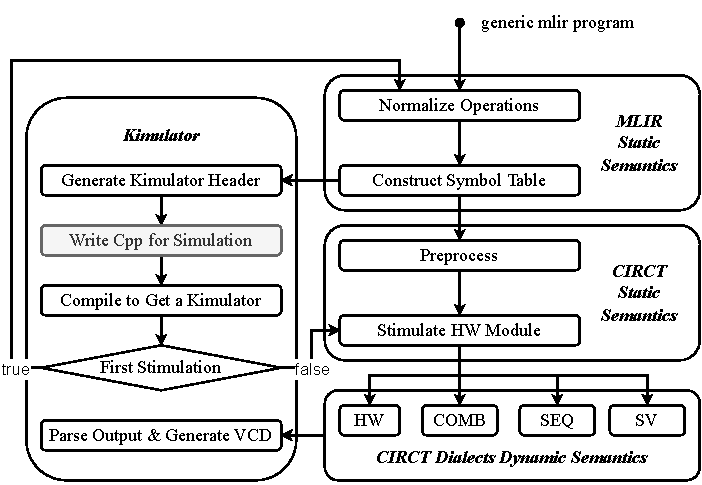
\includegraphics{fig/structure.pdf}
    \caption{The structure of K-CIRCT}
    \label{fig:structure}
\end{figure}

\smallskip
\textbf{Extensible CIRCT Semantics.}
These semantics are structured into three distinct definitions: (1) MLIR static semantics, (2) CIRCT static semantics, and (3) CIRCT dialects dynamic semantics. 

First, the MLIR-level definition serves as a dialect-agnostic semantic representation, conveying essential syntax applicable to any generic MLIR program. This universality ensures compatibility with all MLIR-based applications. Furthermore, we normalize operations to obtain uniform structure, enabling dialect semantics to focus on operation behavior rather than syntax differences. In addition, we construct a symbol table within MLIR semantics, facilitating dialect semantics to access operations based on their symbol names.


% maybe the pre-process should be in the MLIR Semantics? 
% Not: because this is not a concept of MLIR, and not all the dialects need this phase.
Second, CIRCT static semantics define the CIRCT-specific phases that drive the stimulation of all the other dialects within CIRCT. The semantics first introduce the pre-processing phase for operations executed before stimulation, such as macro operations that alter the content of the hardware module. To enable the pre-processing of CIRCT dialects without integrating their semantics into the CIRCT-level semantics, we present control components within the CIRCT-level semantics which the dialect semantics can use to launch their pre-processing. Following pre-processing, the semantics transition to the stimulation phase, where we locate a specific hardware module by searching for its symbol name in the symbol table and then inject the input values into the module.

Thirdly, each CIRCT dialect has its own distinct semantics, enabling independent definitions of operations for extensibility. The prior phases pave the way for dialect semantics to concentrate on their specific concepts, including operations, types, and attributes. We have established the core dialects of CIRCT, including HW, COMB, SEQ, and SV, facilitating the simulation and verification of arbitrary hardware designs compiled using CIRCT, as CIRCT compiles into these dialects.


Consequently, we establish the semantics for \red{???} operations of CIRCT, with corresponding statistics provided in Table~\ref{tab:statistics}. The table's rows denote various metrics, including source lines of code (SLOC), comment lines of code (CLOC), cell count (N cells), rule count (N rules), auxiliary rule count (N aux), and operation count (N ops). The columns consist of MLIR static semantics, CIRCT static semantics, and dynamic semantics for HW, COMB, SEQ, and SV, culminating in the total size.

\begin{table}[!h]
    \centering
    \begin{tabular}{c|c|c|c|c|c|c|c}
               & MLIR & CIRCT & HW & COMB & SEQ & SV & Total \\ \hline
       SLOC    & \red{???} & \red{???} & \red{???} & \red{???} & \red{???} & \red{???} & \red{???} \\ 
       CLOC    & \red{???} & \red{???} & \red{???} & \red{???} & \red{???} & \red{???} & \red{???} \\ 
       N cells & \red{???} & \red{???} & \red{???} & \red{???} & \red{???} & \red{???} & \red{???} \\ 
       N rules & \red{???} & \red{???} & \red{???} & \red{???} & \red{???} & \red{???} & \red{???} \\ 
       N aux & - & - & \red{???} & \red{???} & \red{???} & \red{???} & \red{???} \\
       N ops & - & - & \red{???} & \red{???} & \red{???} & \red{???} & \red{???} \\ 
    \end{tabular}
    \caption{Some statistics for our semantics.}
    \label{tab:statistics}
\end{table}

\smallskip
\textbf{Kimulator for Enhanced Usability.}
Hardware developers commonly use programming languages to simulate hardware and produce VCD files for result analysis. However, the $\mathbb{K}$ framework, a versatile formal framework, does not provide this domain-specific solution.

Thus, we present the kimulator, a tool to enhance the user experience of K-CIRCT. This tool offers a user-friendly interface akin to Verilator, allowing users to write C++ code for simulation and produce VCD files as output. To achieve this, we first develop C++ headers to provide various functions using formal semantics, including modifying input, launching semantics execution, and extracting output. Notably, we manipulate the input and output in Kore language, allowing the generated executor to continue its execution as time progresses, facilitating multiple stimulations. Then, we extend the MLIR static semantics to generate specific headers for hardware modules to be simulated.


\smallskip
\textbf{Validation for Ensured Trustworthiness.} Based on the kimulator, validation is pivotal for establishing the trustworthiness and reliability of K-CIRCT. In pursuit of this goal, we employ a comparative approach by feeding identical inputs into both kimulator and verilator to engage in co-simulation. This co-simulation process is executed in two phases: (1) \textit{Operation-Level Validation}: In this phase, we analyze individual operations to ensure their correctness and functionality. \red{(2) \textit{Hardware-Level Validation}: In the subsequent phase, we expand our validation scope to encompass combinations of instructions, simulating real-world hardware scenarios. This comprehensive approach ensures the robustness and completeness of K-CIRCT.}

\smallskip
\textbf{Summary}. In conclusion, we introduce K-CIRCT, an extensible, user-friendly, and trustworthy framework for CIRCT. This framework is built upon a foundation of hierarchical, isolated, and composable semantics, simplifying maintenance and enabling seamless expansion. The included semantics, such as HW, COMB, SEQ, and SV, not only demonstrate its extensibility but also enhance the usability of CIRCT for simulation and verification purposes. To facilitate practical experimentation and improve user experience, we present the Kimulator, featuring an intuitive C++ interface. To establish the trustworthiness of K-CIRCT, we conduct a comprehensive validation of its semantics through co-simulation. 






